% !Mode:: "TeX:UTF-8" (encoding info for WinEdt)
\section{Verbindung zu externer Datenbank}
Elexis erstellt standardmässig beim ersten Start eine lokale \index{Server!Hsql}HSQL-Datenbank. Man kann aber ohne weiteres auch zu einer anderen Datenbank lokal oder auf einem anderen Computer verbinden, sogar übers Internet (auch wenn das aus Sicherheitsgründen nur mit speziellen Massnahmen empfehlenswert ist)

Erstellen Sie zunächst eine leere Datenbank auf dem Computer, der als Server dienen soll. Wir nehmen mal an, der Server habe die Adresse 192.168.0.2. Für MySQL sind die notwendigen Schritte hier aufgeführt, bei anderen Datenbanken geht es analog.

\subsection{Datenbank anlegen}
\index{Server!Verbindung mit Mysql-Datenbank}
Loggen Sie sich auf dem server ein, und geben Sie auf einer Konsole folgendes ein:

\begin{quote}
mysql -u root
\end{quote}

darauf öffnet sich die mysql-Konsole (Wenn Sie mysql korrekt installiert haben).
Geben Sie dort ein:

\begin{quote}
create database elexistest;

grant all on elexis.* to testuser@'\%' identified by 'testelexis';
\end{quote}

(Es ist natürlich nicht verboten, einen anderen Datenbanknamen und andere Benutzernamen und Passwörter zu nehmen)

Starten Sie dann Elexis und wählen Sie im Menu Datei -> Verbindung.

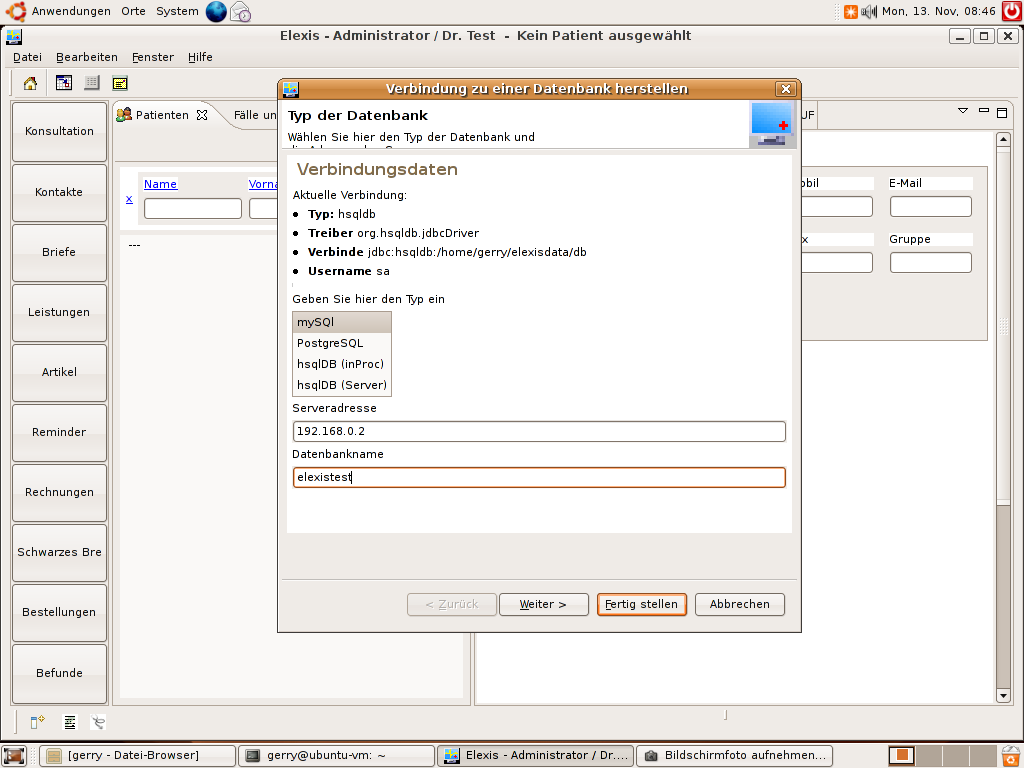
\includegraphics[width=4in]{images/verbindung11.png}
% verbindung11.png: 1024x768 pixel, 72dpi, 36.12x27.09 cm, bb=0 0 1024 768



Geben Sie den Typ der Datenbank (hier mysql), die Adresse des Servers (hier 192.168.0.2) oder dessen Internet-Namen (z.B. testserver.elexis.ch) ein, sowie den Namen der Datenbank (hier  elexistest) ein und klicken Sie auf \textit{weiter}.

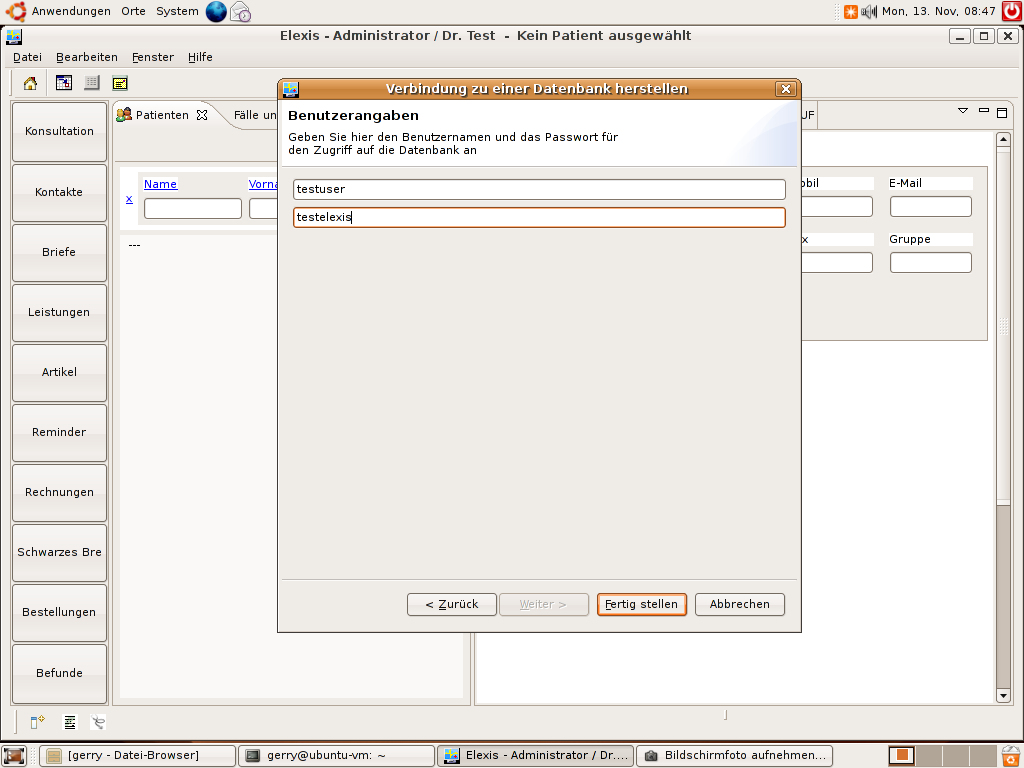
\includegraphics[width=4in]{images/verbindung12.png}
% verbindung12.png: 1024x768 pixel, 72dpi, 36.12x27.09 cm, bb=0 0 1024 768
Geben Sie hier in der oberen Zeile den Benutzernamen für die Datenbank (hier testuser) ein, in die untere Zeile das passende Passwort (hier testelexis) und klicken Sie auf \textit{fertig stellen}.

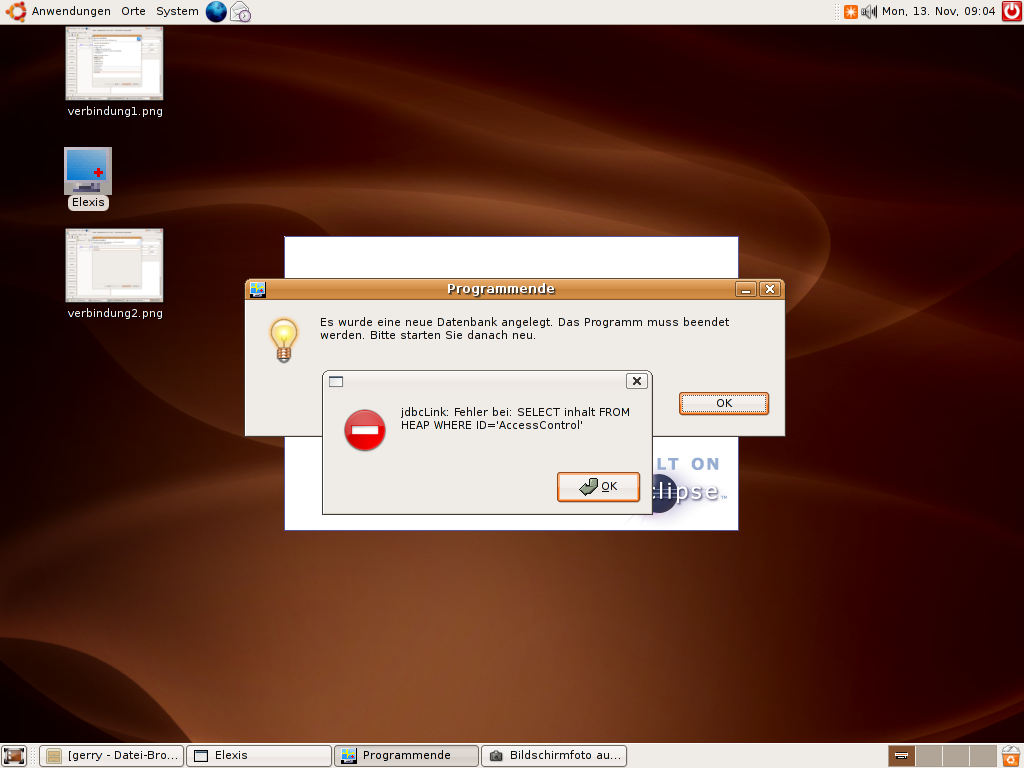
\includegraphics[width=4in]{images/verbindung13.png}
% verbindung13.png: 1024x768 pixel, 72dpi, 36.12x27.09 cm, bb=0 0 1024 768

 Es erscheinen einige Fehlermeldungen, die Sie wegklicken können. Danach müssen Sie das Programm nochmals neu starten.

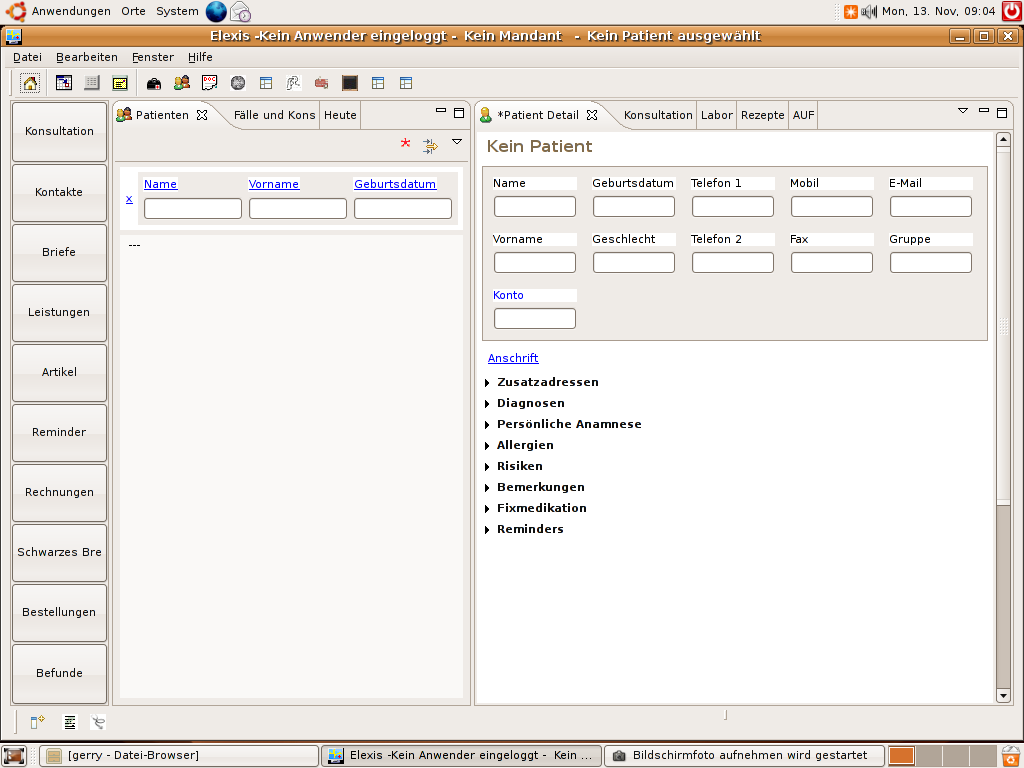
\includegraphics[width=4in]{images/verbindung14.png}
% verbindung14.png: 1024x768 pixel, 72dpi, 36.12x27.09 cm, bb=0 0 1024 768

Sie können sich jetzt mit dem Namen \textit{Administrator} und dem Passwort \textit{admin} an ihrem eben erstellten Elexis-System anmelden.


